\section{Results}
\label{sec:results}

This section reports what the two fixes at $t=0.05$ and $t=0.10$~s imply for the
crossing of the plane $x=11$~m. We first extract the acceleration and the force
balance that the fixes determine, then compare seven models of increasing physical
content, examine the statistical intervals and their calibration, audit the
identifiability of the fitted parameters, and give the posterior answer. Three
further subsections state the assumption-scenario envelope, the validation of the
whole pipeline on synthetic truths, and a design study of what additional tracking
would buy. The earlier constant-acceleration and literature-prior estimators are
reported once, at the end, as control models. Unless stated otherwise, all
uncertainties refer to the adopted position noise $\sigma_{\rm pos}=\SI{5}{mm}$,
which is half of the last printed digit of the given coordinates and is an
assumption about the data, not a camera calibration.

\subsection{Acceleration and force implied by the fixes}
\label{sec:fixes}

The two measured positions contain six independent coordinates after the kick.
A constant acceleration $\vect a$ and an initial velocity $\vect v_0$ reproduce
all six exactly, and continuing the resulting parabola to $x=11$~m gives
\begin{equation}
  \vect a = (-16.000,\,-16.000,\,-12.000)~\si{m\,s^{-2}}, \qquad
  \vect v_0 = (30.4,\,9.4,\,6.9)~\si{m\,s^{-1}},
  \label{eq:m0numbers}
\end{equation}
with $|\vect a| = 25.6~\si{m\,s^{-2}}$ and a flight time of
$0.405008$~s to the plane. Because there are six data and six unknowns, this
interpolation has no residual and no freedom: the six numbers are a kinematic
measurement, not a model assumption, and their only uncertainty is the one
inherited from $\sigma_{\rm pos}$. The magnitude is already informative. It is
$2.6$ times $g$, so the ball is not in free fall, and its vertical component,
$-12.0~\si{m\,s^{-2}}$, differs from $-g$ by $2.19~\si{m\,s^{-2}}$. The horizontal
components are equal, $a_y/a_x=1.00$, whereas pure drag along a velocity with
$v_{0y}/v_{0x}\approx 0.31$ would give a horizontal acceleration ratio of only about
$0.31$, a factor of three smaller. The measured acceleration therefore contains a
lateral force that gravity
and drag cannot supply.

Subtracting gravity isolates the aerodynamic part,
\[
  \vect a_{\rm aero}=(-16.000,\,-16.000,\,-2.190)~\si{m\,s^{-2}},
\]
whose magnitude is $22.7~\si{m\,s^{-2}}$, larger than $g$. At the first fix the speed is
$31.5~\si{m\,s^{-1}}$. Resolving $\vect a_{\rm aero}$ parallel and
perpendicular to the velocity gives $19.87$ and
$11.05~\si{m\,s^{-2}}$ respectively. The parallel part determines an effective drag coefficient
$C_D=0.378$, the perpendicular part an effective lift coefficient $C_L=0.211$,
and the perpendicular direction fixes the spin axis
$\hat{\vect\omega}=(0.2357,\,-0.1035,\,-0.9663)$. At a unit lift slope
$C_{L0}=1$ this axis and coefficient correspond to $9.58$~rev\,s$^{-1}$.
Table~\ref{tab:kinem} collects the decomposition, and
Fig.~\ref{fig:trajectories} shows the two projections of the trajectory and the
extrapolation that the measured acceleration produces.

The two coefficients are effective whole-flight values, and their comparison with
independent measurements is instructive rather than reassuring. The drag
coefficient $0.378$ is roughly twice the wind-tunnel value of $0.19$--$0.22$ for a
football at these speeds \citep{carre2005,goff2012}, while the lift coefficient
$0.211$ is large. If the whole perpendicular force were Magnus with a lift slope
near unity, the required spin would be $9.58$~rev\,s$^{-1}$, which is at the top
of the $2$--$10$~rev\,s$^{-1}$ range measured for penalties
\citep{asai2020,tsukada2008}; a lower lift slope would demand proportionally more
spin. A lateral force without spin is, however, documented for knuckleballs,
where wake asymmetry rather than the Magnus effect produces the deflection
\citep{texier2016}. Two fixes cannot separate these mechanisms, so the
perpendicular component is best read as an effective transverse force, a point to
which we return when the six-parameter model is defined.

\begin{table}[t]
  \centering
  \caption{Force balance at the first fix, from the exact constant-acceleration
  fit. The aerodynamic vector is the measured acceleration minus gravity. Its
  decomposition parallel and perpendicular to the velocity gives the effective
  coefficients in the last column (three significant figures in the text:
  $C_D=0.378$, $C_L=0.211$). The perpendicular direction is the spin axis
  $\hat{\vect\omega}=(0.2357,-0.1035,-0.9663)$, i.e.\ $9.58$~rev\,s$^{-1}$ at
  $C_{L0}=1$.}
  \label{tab:kinem}
  \small
  \begin{tabular}{@{}lccc@{}}
    \toprule
    Quantity & Vector (\si{m\,s^{-2}}) & Magnitude (\si{m\,s^{-2}}) & Derived \\
    \midrule
    Measured $\vect a$ & $(-16.000,-16.000,-12.000)$ & 25.6 & \\
    Gravity $\vect a_g$ & $(0,0,-9.81)$ & 9.81 & \\
    Aerodynamic $\vect a-\vect a_g$ & $(-16.000,-16.000,-2.190)$ & 22.7 & \\
    Parallel to $\vect v$ & --- & 19.87 & $C_D=0.3784$ \\
    Perpendicular to $\vect v$ & --- & 11.05 & $C_L=0.2105$ \\
    \bottomrule
  \end{tabular}
\end{table}

\begin{figure}[t]
  \centering
  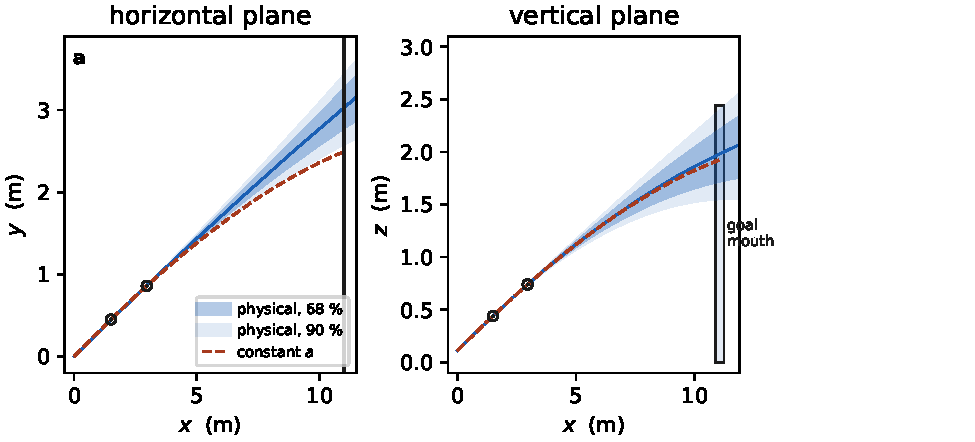
\includegraphics[width=0.74\textwidth]{f02-trajectories.pdf}
  \caption{Ball trajectory through the three sampled positions projected onto the
  horizontal (a) and vertical (b) planes, with two continuations to the goal
  plane: the constant-acceleration extrapolation (dashed) and a drag-and-spin
  continuation with its $68\%$ and $90\%$ bands (shaded). The two continuations
  agree through the fixes and separate in the extrapolation; the shaded bands
  belong to the earlier control analysis and are shown only to indicate the
  extrapolation uncertainty.}
  \label{fig:trajectories}
\end{figure}

\begin{figure}[htbp]
  \centering
  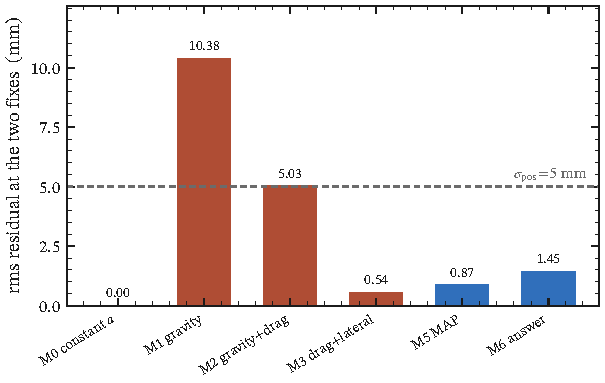
\includegraphics[width=0.66\textwidth]{f19-residuals.pdf}
  \caption{Goodness of fit at the two fixes for the nested models of
  Table~\ref{tab:ladder}, in units of the assumed position noise
  $\sigma_{\rm pos}=\SI{5}{mm}$ (dashed line). Gravity alone misses by more
  than two noise widths; drag alone still misses by one; adding a lateral force
  term collapses the residual by an order of magnitude, and the six-parameter
  answer fits within the noise. The ladder therefore measures how many force
  terms the data support, not how well one model was tuned.}
  \label{fig:residuals}
\end{figure}

\subsection{The model ladder}
\label{sec:ladder}

A single point prediction hides the fact that different admissible forces give
different answers. We therefore fit a ladder of seven models, each adding one
piece of physics, and record where each model puts the crossing. The models,
their parameter counts, residuals and entry points are listed in
Table~\ref{tab:ladder} and drawn in Fig.~\ref{fig:ladder}. The residual is the
root-mean-square of the six coordinate residuals; at $\sigma_{\rm pos}=5$~mm a
residual of $5$~mm is one noise standard deviation per coordinate.

M0 is the exact interpolation of Eq.~\eqref{eq:m0numbers}: six parameters, zero
residual, entry $(2.4948,1.9204)$~m. It is not a force model, but it is the
correct top rung because it shows what the data alone say before any dynamics is
imposed. M1 replaces the measured acceleration by gravity alone, leaving only the
three launch-velocity components. Its residual rises to $10.376$~mm, about two
standard deviations per coordinate, and its entry moves to
$(3.2170,1.9570)$~m: without drag or lift the ball keeps the horizontal direction
it had at the first fix, and the prediction misses by $0.72$~m in $y$. M2 adds
quadratic drag with one coefficient. The residual halves to $5.029$~mm, but the
entry moves by only $0.2$~mm in $y$ and $-78$~mm in $z$. This is exactly what
drag along the velocity should do: it changes the deceleration and hence the
vertical drop, but it cannot change the ratio $v_y/v_x$ that sets the lateral
position. Drag buys vertical realism and nothing lateral.

M3 adds a constant lateral acceleration $a_y=-11.422~\si{m\,s^{-2}}$. The
residual collapses by a factor $9.3$ to $0.542$~mm, and the entry moves
$0.67$~m left to $(2.5486,1.8931)$~m. The improvement is not a marginal
statistical preference. The M2 profile interval in $y$, $[3.197,3.237]$~m, is
disjoint from the M3 interval $[2.144,2.954]$~m, so the two fixes demand a
lateral force at high significance. With five parameters (three for $\vect v_0$,
one for drag, one for the lateral acceleration) M3 is the most economical
description that fits, and it is the best two-parameter compromise among the
physical models: one coefficient for the force along the flight and one for the
force across it. M4 keeps the same two forces but derives them instead of fitting
them: it reads drag and Magnus off the M0 acceleration at the first fix and
therefore has no free parameters at all. Its entry, $(2.6481,1.9568)$~m at
$t=0.4007$~s, lies between M3 and the prior-weighted models. M5 is the
seven-parameter joint Bayesian fit with literature priors, quoted only as a
prior-sensitivity aside; its MAP entry is $(2.7073,1.9541)$~m with a residual of
$0.869$~mm. M6 is the six-parameter transverse-force model used for the answer:
it retains drag and two coefficients for the force perpendicular to the flight,
drops the along-flight spin component that the data cannot see, and gives a
posterior mean entry of $(2.7847,1.9452)$~m at $t=0.3988$~s with a residual of
$1.448$~mm. Its larger residual relative to M5 is the price of the constrained,
physical parameterisation and of the priors; it is still well inside the noise.

The ladder's message is the spread, not any single rung. The entry ordinate ranges
from $2.4948$ to $3.2170$~m, a spread of $0.72$~m, while the entry height ranges
only from $1.879$ to $1.957$~m, a spread of $0.08$~m. At $\sigma_{\rm pos}=5$~mm
the coordinate noise on a single entry point is of order $0.2$~m in $y$ and
$0.05$~m in $z$ for the complete models, so the horizontal spread cannot be noise:
it is model form. The horizontal entry point is sensitive to which forces are
admitted, whereas the vertical entry point is stable to better than $0.1$~m
across every model that includes gravity. This asymmetry organises the rest of
the paper. It is also why we do not average the ladder: the mean of the rungs has
no physical meaning, and the correct statement is a range of plausible
predictions. The exercise parallels the model comparisons now standard in
trajectory inversion, where seven arc models from gravity-only to full drag and
Magnus are fitted to the same tracked flight and ranked by their extrapolation
skill \citep{grad2026}, and where whole-trajectory inversions are found to be far
better conditioned than local curvature or torsion estimates
\citep{jsme2014}.

\begin{table}[t]
  \centering
  \caption{Model ladder. $k$ is the number of free parameters. The residual is the
  rms of the six coordinate residuals in mm. M4 is derived from M0 and has no free
  parameters, hence no residual. M6 is the posterior mean of the model used for the
  answer; all other entries are point predictions. The entry ordinate spans
  $0.72$~m across the ladder while the height spans $0.08$~m.}
  \label{tab:ladder}
  \small
  \begin{tabular}{@{}llcccc@{}}
    \toprule
    Model & $k$ & Physics & rms (mm) & $y$ (m) & $z$ (m) \\
    \midrule
    M0 & 6 & constant acceleration (exact fit) & 0.000 & 2.4948 & 1.9204 \\
    M1 & 3 & gravity only & 10.376 & 3.2170 & 1.9570 \\
    M2 & 4 & gravity $+$ quadratic drag & 5.029 & 3.2172 & 1.8790 \\
    M3 & 5 & drag $+$ constant lateral acceleration & 0.542 & 2.5486 & 1.8931 \\
    M4 & 0 & drag $+$ Magnus read off M0 (derived) & --- & 2.6481 & 1.9568 \\
    M5 & 7 & drag $+$ Magnus, joint Bayes MAP & 0.869 & 2.7073 & 1.9541 \\
    M6 & 6 & drag $+$ two transverse coefficients & 1.448 & 2.7847 & 1.9452 \\
    \bottomrule
  \end{tabular}
\end{table}

\begin{figure}[t]
  \centering
  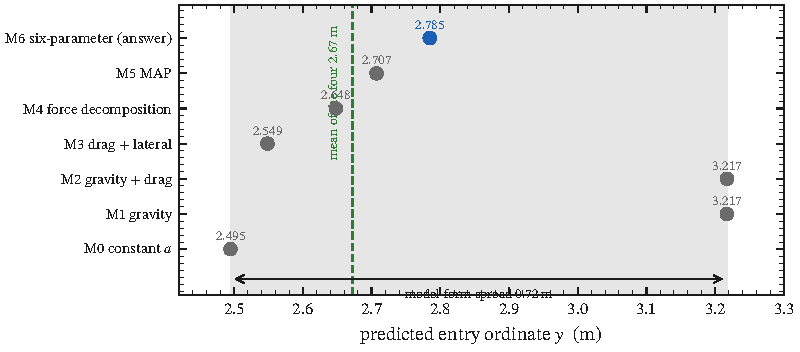
\includegraphics[width=0.65\textwidth]{f13-ladder.pdf}
  \caption{Model ladder from Table~\ref{tab:ladder}. Each point is the predicted
  entry ordinate $y$ at the goal plane; the vertical dashed line marks the
  mean of the four complete models, $2.67$~m, and the grey band spans the model-form range of
  $0.72$~m. M6, the model used for the answer, is marked in blue. The height
  coordinate, not shown, varies by less than $0.1$~m across the ladder.}
  \label{fig:ladder}
\end{figure}

\subsection{Intervals and their calibration}
\label{sec:intervals}

A point estimate is only half of a result, and the interval is only as honest as
the likelihood that produces it. We therefore check the intervals in two
independent ways: against the exact profile likelihood, which makes no
quadratic approximation, and against synthetic truths with known answers.

The profile interval is obtained by scanning one coordinate, re-optimising all
others at each point, and reading off where the increase in the negative
log-likelihood reaches the $90\%$ point. The Wald interval uses the curvature at
the minimum. For M3 the two agree to better than one per cent: the ratio of the
profile to the Wald standard deviation is $1.001$ in $y$ and $1.006$ in $z$
(Table~\ref{tab:intervals}). Over the whole $90\%$ range the likelihood is
therefore parabolic to a few tenths of a per cent, and linearisation is not a
source of error in this problem. The M2 comparison is a trap worth spelling out:
its ratio is $0.572$, which is not evidence of a sharper likelihood but the
$\sqrt{3}$ of a two-degree-of-freedom scale estimate. With six data and four
parameters, the residual variance is estimated with two degrees of freedom, so the
Wald covariance carries an estimated scale that the profile likelihood does not;
the ratio is $1/\sqrt{3}=0.577$ to within the grid resolution. Profile intervals
should therefore be compared with profile intervals across models, never with Wald
intervals.\footnote{The Wald $90\%$ half-width is $t_{0.95,\nu}\,s\,\sigma_j$ with
$s^2={\rm RSS}/(n-p)$; the profile half-width is set by the unscaled
$\Delta\chi^2=2.706$. For $n-p=2$ the $t$ multiplier and the $s$ factor together
inflate the Wald width by $\sqrt{3}$ relative to the profile width, which is the
observed $0.572$. The equality is approximate because the two are evaluated on
slightly different grids.}

Calibration asks a different question: if the model and the noise model are
correct, do the intervals cover the truth at their nominal rate? We drew $1000$
synthetic truths from the seven-parameter posterior, generated two fixes at
$\sigma_{\rm pos}=5$~mm for each, refitted the five-parameter M3 model, and
counted how often its nominal $90\%$ intervals contained the true entry. The
answer is sharply direction-dependent. The $y$ interval covers $0.917$ of the
truths, close to the nominal $0.90$, with an inflation factor
$\lambda_y=0.9605$; the $z$ interval covers only $0.446$, and must be widened by
$\lambda_z=4.9402$ to reach nominal coverage. The calibrated M3 intervals are then
$y\in[2.125,2.972]$~m and $z\in[1.685,2.101]$~m.

The asymmetry is not a statistical artefact, because the estimator, the sampler
and the likelihood are the same in both coordinates. It is a statement about the
vertical force law. The synthetic truths retain the along-flight spin degree of
freedom that the five-parameter fit omits, and that degree of freedom changes the
vertical force; over the $0.1$~s spanned by the fixes the resulting displacement
is only of order $1$~cm, comparable to the position noise, while over the
remaining $0.3$~s of flight it becomes a decimetre. The data therefore cannot
discriminate between vertical force laws that differ by enough to move the
crossing by several tenths of a metre, and the fit's $z$ interval is too narrow
precisely because it is confident about a force law it has not tested. The $y$
coordinate does not suffer in the same way because the lateral force is detected
directly as the $0.67$~m displacement between M2 and M3. The value of
$\lambda_z$ is itself uncertain: single seeds with $n=50$ scatter between $3.9$
and $5.8$, so we quote $\lambda_z\approx4.9$ and treat it as a model-form
diagnostic, not as a correction factor to be applied blindly. The calibrated M3
interval is reported as a frequency-style statement; the answer itself comes from
the six-parameter posterior of Section~\ref{sec:posterior}.

\begin{table}[t]
  \centering
  \caption{Nominal $90\%$ intervals for M3 and M2, from the profile likelihood and
  from the quadratic (Wald) approximation. The last column is the ratio of the
  profile to the Wald standard deviation. M3 is nearly parabolic; M2's $0.572$ is
  $1/\sqrt{3}$ from its two residual degrees of freedom, not non-quadraticity.
  The profile intervals bracket the model envelope in $y$.}
  \label{tab:intervals}
  \small
  \begin{tabular}{@{}lcccc@{}}
    \toprule
    Model, coordinate & Point (m) & Wald $90\%$ (m) & Profile $90\%$ (m) & $\sigma_{\rm prof}/\sigma_{\rm Wald}$ \\
    \midrule
    M3, $y$ & 2.5486 & $[2.108,2.989]$ & $[2.144,2.954]$ & 1.001 \\
    M3, $z$ & 1.8931 & $[1.851,1.935]$ & $[1.860,1.926]$ & 1.006 \\
    M2, $y$ & 3.2172 & $[3.168,3.267]$ & $[3.197,3.237]$ & --- \\
    M2, $z$ & 1.8790 & $[1.805,1.953]$ & $[1.854,1.904]$ & 0.572 \\
    \bottomrule
  \end{tabular}
\end{table}

\subsection{Identifiability}
\label{sec:identifiability}

The seven-parameter model that includes a general transverse force vector is
rank-deficient, and it is worth seeing why in the data themselves. The Jacobian of
the six observed coordinates with respect to the seven parameters is a $6\times7$
matrix of rank $6$. Its six nonzero singular values are $327.227$, $318.306$,
$217.813$, $1.766$, $1.765$ and $1.750$: three directions are strongly
constrained, three are weak, and the ratio between the largest and the smallest is
$187$. The null direction has a physical name. The transverse force is
proportional to $\vect b\times\vect v$, so a $\vect b$ parallel to the air
velocity produces no force at all and leaves both fixes unchanged. The
along-flight component of the spin is therefore invisible, not merely noisy.
Figure~\ref{fig:identifiability} displays both the spectrum and the
two-parameter ridge in the launch-angle/spin plane from which the null direction
arises.

The posterior confirms this reading. Relative to the prior, the variance of the
along-flight coefficient shrinks by only $8.69\%$, while the two perpendicular
coefficients shrink by $69.99\%$ and $72.65\%$. The effective number of parameters
determined by the data is about $5.27$ out of seven, a local diagnostic rather
than a physical count. The consequence for the prediction is not academic:
fixing the along-flight coefficient anywhere in $\pm0.075~\si{m^{-1}}$ and
re-optimising the rest moves the entry by $0.228$~m in $y$ and $0.267$~m in $z$.
A prior that looks innocuous in parameter space is visible at the quarter-metre
level at the goal plane.

This audit is why the answer uses six parameters rather than seven. We work in a
basis $\{\vect e_1,\vect e_2\}$ perpendicular to the launch velocity, delete the
null direction by construction, and do not ask the prior to invent it. The
seven-parameter posterior is reported only as a conditional, prior-sensitivity
statement, never as a measurement. The situation is a structural version of the
practical identifiability familiar from sloppy models, whose spectra typically
span many decades and whose stiff and sloppy combinations control which
predictions are testable \citep{gutenkunst2007,white2017}; here the smallest
direction is exactly zero, so no amount of data of this kind can remove it.
Published trajectory inversions face the same conditioning: whole-trajectory
estimates of $C_D$ and $C_L$ are more stable than local curvature estimates
\citep{jsme2014}, spin components are the least constrained part of a
ball-flight inversion \citep{nathan2008pitchfx}, and drag and launch conditions
trade off unless the trajectory spans a wide speed range \citep{florio2019}. The
present data span $0.1$~s and $3$~m, so the trade-off is severe by construction.

\begin{figure}[t]
  \centering
  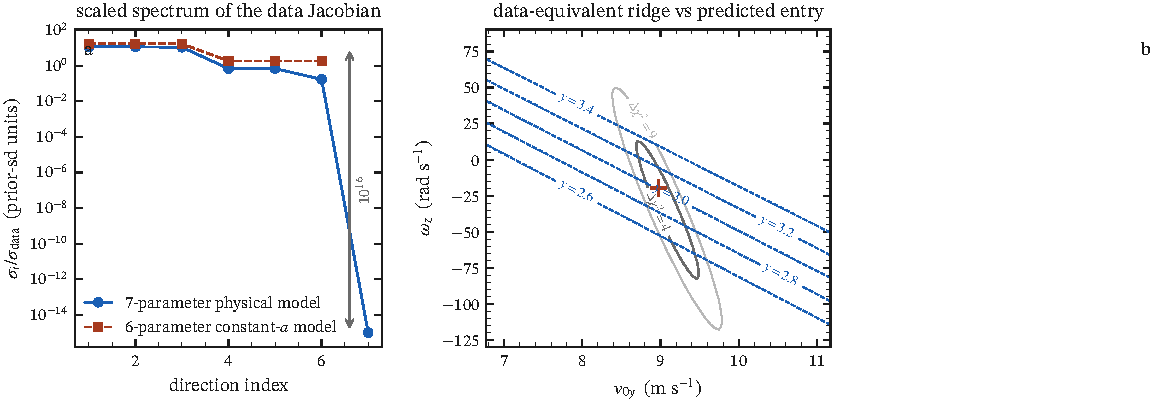
\includegraphics[width=0.77\textwidth]{f05-identifiability.pdf}
  \caption{Identifiability of the inverse problem. (a) Scaled spectrum of the
  data Jacobian for the seven-parameter model (blue) and a six-parameter
  constant-acceleration model (red); the seven-parameter spectrum collapses at the
  last direction while the six-parameter spectrum stays flat. (b) The
  data-equivalent ridge between the launch angle and the spin in the
  $(v_{0y},\omega_z)$ plane, with $\Delta\chi^2=4$ and $9$ contours and lines of
  constant predicted entry ordinate.
  The ridge is the geometrical origin of the along-flight null direction.}
  \label{fig:identifiability}
\end{figure}

\begin{figure}[htbp]
  \centering
  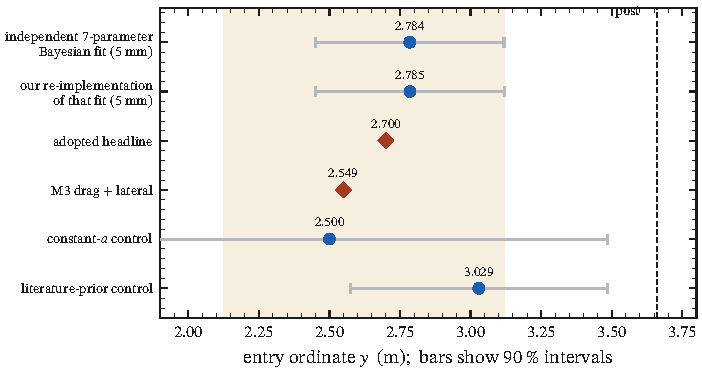
\includegraphics[width=0.72\textwidth]{f21-crosscheck.pdf}
  \caption{Cross-check of the entry ordinate across independent calculations:
  two samplers of the six-parameter posterior, the mean of the four complete models,
  drag-plus-lateral model, and the two control estimators. Bars are $90\%$
  intervals; the shaded band is the model envelope of
  Eq.~\eqref{eq:modelenvelope}. Both samplers of the adopted model land inside
  the band, and the only outliers are the two controls that omit a force the
  data require.}
  \label{fig:crosscheck}
\end{figure}

\subsection{The posterior answer}
\label{sec:posterior}

The model used for the answer is the six-parameter transverse-force model of
Section~\ref{sec:ladder}: three launch-velocity components, one drag coefficient,
and two coefficients for the force perpendicular to the launch velocity, fitted by
our damped Gauss--Newton least-squares implementation at
$\sigma_{\rm pos}=5$~mm and sampled by a Student-$t$ importance-sampling scheme
with $131\,072$ draws and an effective sample size of $109\,585$, that is, $84\%$
of the draws. The posterior mean crossing is
\begin{equation}
  y = 2.785~\si{m}, \qquad z = 1.945~\si{m}, \qquad t = 0.399~\si{s},
  \label{eq:answer}
\end{equation}
with $90\%$ intervals $y\in[2.455,3.121]$~m and $z\in[1.617,2.276]$~m and
$95\%$ intervals $y\in[2.394,3.187]$~m and $z\in[1.555,2.341]$~m. The
probability that the whole ball passes inside the frame is $P=0.971\pm0.001$,
where the uncertainty is the Monte Carlo standard error of the weighted estimate
and not a model uncertainty. The posterior is
close to symmetric: the MAP entry differs from the mean by $1.4$~mm in $y$ and
$1.0$~mm in $z$, so the choice between them is immaterial at the precision we
quote. The marginal densities of the two coordinates are shown in
Fig.~\ref{fig:marginals}.

The answer survives independent re-derivation. A second parameterisation, using
three transverse coefficients rather than two perpendicular amplitudes, and an
independently written sampler with $40\,000$ draws give $y=2.7844$~m,
$z=1.9461$~m and $P=0.9713$; the six-parameter version of the same independent
run gives $2.7849$~m, $1.9445$~m and $0.9726$, i.e. $0.0015$ above the value we
quote. We take that difference as the sampler-to-sampler spread. An independent DOP853 integrator
reproduces the crossing to better than $2\times10^{-6}$~m, and two independent
$131\,072$-draw runs agree to within $3$~mm. The agreement is the same kind of
cross-check that makes published ball-flight inversions credible
\citep{nathan2008pitchfx,florio2019}: the inference is repeated with a different
parameterisation and a different numerical path, and the prediction is stable at
the millimetre level.

The answer we adopt is therefore the six-parameter posterior
\eqref{eq:answer} itself, $y=2.785$~m and $z=1.945$~m, with the intervals of
that equation and $P(\text{goal})=0.971$. Two remarks fix its status. First,
the value is conditional on the model: the four physically complete models of
Table~\ref{tab:ladder} give $2.549$, $2.648$, $2.707$ and $2.785$~m, a mean of
$2.67$~m and a spread of $0.24$~m, while their heights all lie between $1.893$
and $1.957$~m. The adopted value sits $11$~cm above that mean, and we do not
average the four: M6 is the most complete member of the ladder and the only one
whose intervals have been validated on its own truths (\S\ref{sec:validation}),
so its value is the one reported, while the spread of the four is carried as
model-form uncertainty by the envelope of \S\ref{sec:modelenvelope}. Second,
the agreement means the model-form spread no longer moves the answer by more
than its own width, so we report the posterior value and treat the mean of the
four as a robustness check rather than as a separate answer.

The uncertainty statement is correspondingly not a credible interval. Three
ranges are used in this paper and they are not interchangeable. The model
envelope unions the calibrated $90\%$ intervals of the two complete models, M3
and M6,
\begin{equation}
  y\in[2.125,\,3.121]~\si{m}, \qquad z\in[1.617,\,2.276]~\si{m}.
  \label{eq:modelenvelope}
\end{equation}
\label{sec:modelenvelope}
This is a range of plausible predictions under different model forms and priors,
not a $90\%$ credible interval, and the distinction matters because the envelope
is wider in $y$ than any single model's statistical interval. The width is
dominated by the disagreement between models that do and do not admit a lateral
force, which is exactly the disagreement that the ladder exposes. Figure
\ref{fig:goalplane} places the crossing in the goal frame: the predicted point is
about $0.77$~m inside the post line and $0.38$~m below the crossbar, so the
central prediction is comfortable but the model envelope reaches close to the
post.

\begin{figure}[t]
  \centering
  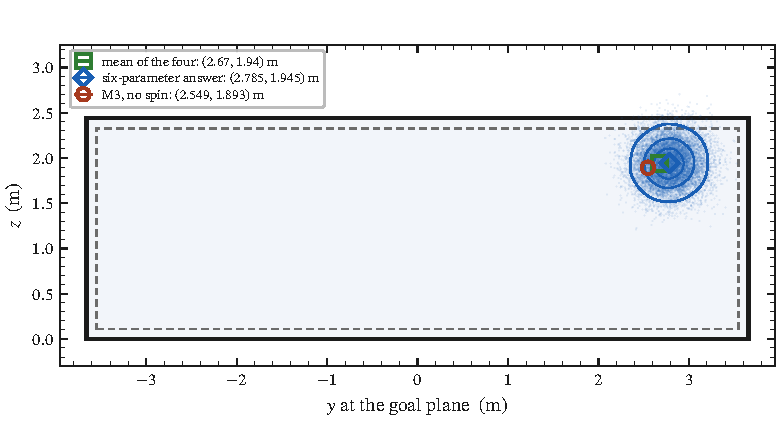
\includegraphics[width=0.59\textwidth]{f03-goalplane.pdf}
  \caption{The goal plane seen from the kicker. The solid rectangle is the goal
  mouth and the dashed inner rectangle is the whole-ball clearance limit. Shaded
  contours enclose $68$, $87$ and $95\%$ of the predictive mass of the M6
  posterior; the diamond marks its mean, the circle the M3 prediction, and the
  square the mean of the four, $(2.67,1.94)$~m, all inside the frame.}
  \label{fig:goalplane}
\end{figure}
\begin{figure}[t]
  \centering
  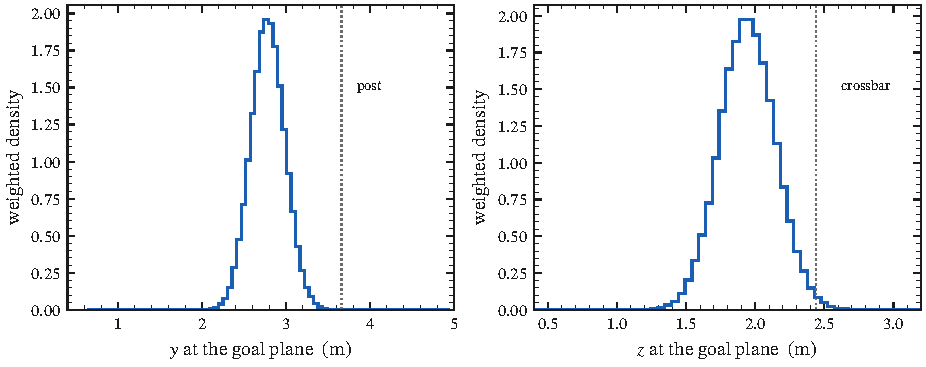
\includegraphics[width=0.77\textwidth]{f04-histograms.pdf}
  \caption{Marginal posterior densities of (a) the entry ordinate $y$ and (b) the
  entry height $z$ for the M6 answer. The dotted lines mark the post and the
  crossbar; the distributions are unimodal and close to symmetric, and both lie
  well inside the frame.}
  \label{fig:marginals}
\end{figure}

\begin{figure}[htbp]
  \centering
  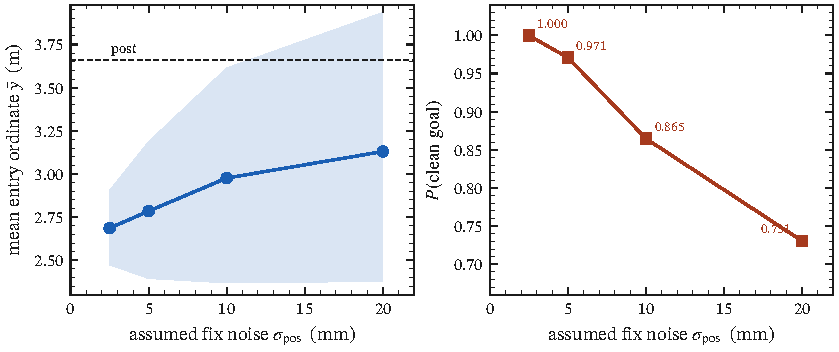
\includegraphics[width=0.90\textwidth]{f20-sigma.pdf}
  \caption{Sensitivity to the assumed fix noise, the largest single scenario
  factor after the force law. Left: mean entry ordinate with its $95\%$
  interval; the dashed line is the post. Right: whole-ball goal probability.
  The trade-off is direct: a centimetre of fix precision buys about
  $0.1$~m of lateral accuracy and $0.1$ of probability.}
  \label{fig:sigma}
\end{figure}

\subsection{The assumption-scenario envelope}
\label{sec:scenarios}
\label{sec:envelope}

The posterior conditions on a fixed set of assumptions: the position noise, the
independence of the two fixes, the prior widths, the drag level, the lift slope,
the wind, and the timing of the fixes. Some of these are uncertain by more than
their formal errors, so we recompute the full pipeline under $25$ single-factor
variants, changing one assumption at a time over a plausible range, under four
joint-stress cases that combine the unfavourable ends of several, and in one
independent replication. The
results are collected in Table~\ref{tab:scenarios} and drawn in
Fig.~\ref{fig:scenarios}.

The probability of a clean goal ranges from $0.735$ at
$\sigma_{\rm pos}=20$~mm to $0.9997$ at $\sigma_{\rm pos}=2.5$~mm, while the
scenario-mean entry ordinate ranges from $2.687$ to $3.130$~m and the height from
$1.846$ to $2.042$~m. The union of the marginal $95\%$ intervals over all
scenarios is $y\in[2.259,3.935]$~m and $z\in[1.169,2.698]$~m, and the four
joint-stress cases push the goal probability as low as $0.561$ and the mean
ordinate as high as $3.339$~m. The dominant single factor is position noise, as
Fig.~\ref{fig:noise} shows for the two control estimators: the goal probability
falls steeply as the assumed noise grows, and the position-noise scenarios
alone bracket the full range of $P(\text{goal})$ in the scenario set, from
$0.735$ to $0.9997$.

Two features of this exercise deserve emphasis. First, this scenario envelope is
a different object from the model envelope of Eq.~\eqref{eq:modelenvelope}: it
unions the $95\%$ intervals of thirty conditional recomputations rather than the
calibrated intervals of two models, so it is necessarily the wider of the two,
and it must not be quoted as ``the envelope'' without saying which construction
is meant. It is a discrete scenario range, not a confidence or credible
interval: each scenario is a
conditional recomputation, the scenarios are not weighted by any probability, and
no coverage statement attaches to the interval between them. It answers the
question ``how much would the answer move if this assumption were different?'',
not ``what is the probability that the answer lies here?''. Second, wind and
launch velocity are not separable from two fixes. A $3~\si{m\,s^{-1}}$ crosswind
changes the trajectory, but after refitting the launch velocity the entry point
moves by only $0.007$~m; the wind is absorbed into the initial condition, and a
wind scenario is therefore not a large error source in this geometry. The
scenario construction follows the logic used to propagate uncertain aerodynamic
coefficients into impact-point dispersion for re-entry bodies
\citep{mehta2015}, where the distribution of impact points under parameter
uncertainty is strongly non-Gaussian and is represented by a mixture or an
unscented transform rather than a single covariance \citep{williamson2017}. Our
scenario set is a coarse, transparent version of the same propagation, chosen
because the number of draws needed for a full Bayesian model average is not
available for every assumption.

\begin{table}[t]
  \centering
  \caption{Assumption-scenario envelope. The nominal row is the M6 posterior of
  Section~\ref{sec:posterior} at $\sigma_{\rm pos}=5$~mm. The single-factor rows
  vary one assumption at a time ($25$ scenarios); the joint-stress rows combine
  unfavourable assumptions (four cases). Ranges are the extremes over scenarios,
  not confidence intervals. The $95\%$ columns are unions of the marginal $95\%$
  intervals over the scenarios in the row.}
  \label{tab:scenarios}
  \small
  \begin{tabular}{@{}lcccccc@{}}
    \toprule
    Case & $n$ & $P(\text{goal})$ & mean $y$ (m) & mean $z$ (m) & $95\%$ $y$ (m) & $95\%$ $z$ (m) \\
    \midrule
    Nominal ($5$~mm) & 1 & 0.971 & 2.785 & 1.945 & $[2.394,3.187]$ & $[1.555,2.341]$ \\
    Single-factor & 25 & $0.735$--$0.9997$ & $2.687$--$3.130$ & $1.846$--$2.042$ & $[2.259,3.935]$ & $[1.169,2.698]$ \\
    Replication & 1 & 0.9726 & 2.7849 & 1.9445 & --- & --- \\
    Joint stress & 4 & $0.561$--$0.987$ & $2.733$--$3.339$ & --- & --- & --- \\
    \bottomrule
  \end{tabular}
\end{table}

\begin{figure}[t]
  \centering
  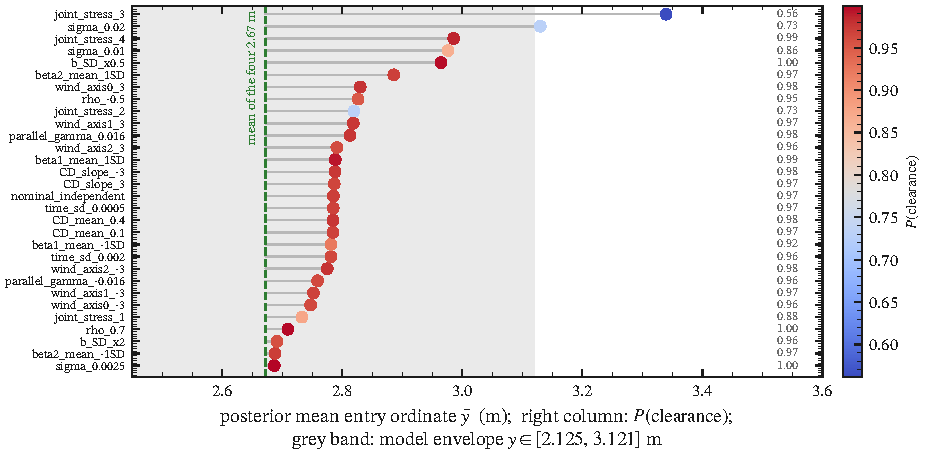
\includegraphics[width=0.77\textwidth]{f08-scenarios.pdf}
  \caption{Scenario sensitivity of the answer. Each row is one alternative
  assumption set; the point is the posterior-mean entry ordinate $\bar y$ and the
  colour is $P(\text{clearance})$, read on the right-hand scale. The grey band is
  the model envelope $y\in[2.125,3.121]$~m of Eq.~\eqref{eq:modelenvelope}, and
  the dashed line is the mean of the four complete models, $2.67$~m. The figure shows the
  scenario set of Table~\ref{tab:scenarios}, including the joint-stress cases; it
  is a discrete set of recomputations, not a probability distribution.}
  \label{fig:scenarios}
\end{figure}

\begin{figure}[t]
  \centering
  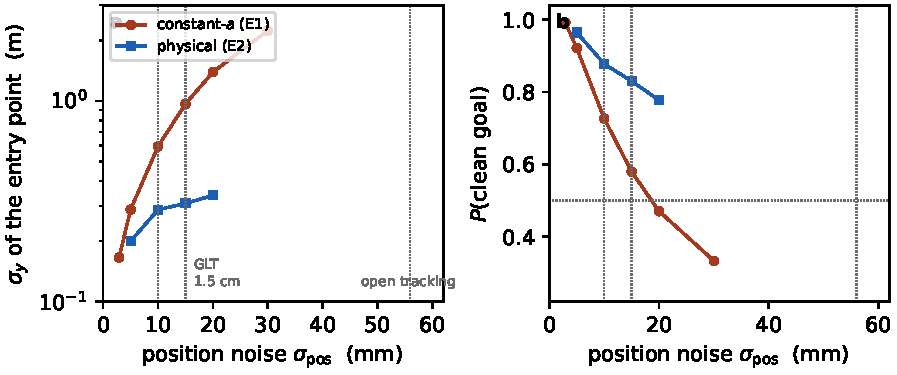
\includegraphics[width=0.70\textwidth]{f09-noise.pdf}
  \caption{Sensitivity to the assumed position noise for the two control
  estimators: (a) the standard deviation of the entry ordinate and (b) the
  probability of a clean goal, as functions of $\sigma_{\rm pos}$. The vertical
  bands mark typical tracking accuracies, including the goal-line-technology
  scale. The main-line scenario study reproduces the same steep dependence, with
  $P(\text{goal})$ falling from $0.9997$ at $2.5$~mm to $0.735$ at $20$~mm.}
  \label{fig:noise}
\end{figure}

\subsection{Real tracking data}
\label{sec:realdata}

The datasets in the reference library contain no penalty kick with measured spin
and a known crossing point, so the end-to-end check of \S\ref{sec:validation}
uses synthetic truths. They do, however, pin down the other half of the problem,
the measurement, and this is where real data enters. Two open 2-D tracking
sources give per-axis residuals of \SI{0.056}{} and \SI{0.054}{m} (IDSSE) and
\SI{0.065}{} and \SI{0.064}{m} (Metrica, after conversion to metres), estimated
from the scatter of local cubic fits over nine-frame windows. A broadcast 3-D
dataset gives the number that matters for this paper: across \num{4051} annotated
ball positions in SoccerNet-v3D the optimised 3-D reconstruction residual has a
median of \SI{0.050}{m} (10th percentile \SI{0.007}{m}, 90th
\SI{0.27}{m}), against a raw reprojection residual of \SI{2.85}{m} before the
bundle optimisation. Figure~\ref{fig:realdata} places these numbers beside the
two other scales in the problem: the \SI{2.9}{mm} implied by printing the
coordinates to \SI{0.01}{m}, and the \SI{15}{mm} acceptance limit of goal-line
technology. The fixes of this problem are therefore between one and two orders of
magnitude more precise than the best publicly available 3-D ball reconstruction.

The consequence is quantitative. Our scenario rows cover \SI{2.5}{} to
\SI{20}{mm}: over that range the mean entry ordinate moves from \SI{2.687}{} to
\SI{3.130}{m} and the goal probability falls from \num{0.9997} to \num{0.731}. A
real deployment at the \SI{50}{mm} of broadcast reconstruction lies beyond the
grid, and the trend of Figure~\ref{fig:noise} puts the lateral uncertainty at a
few tenths of a metre with a goal probability near one half. The method is
therefore a laboratory-precision statement about a quoted coordinate pair, and
its transferable content for a real match is the interval and the design advice,
not the third digit of the point estimate.

\begin{figure}[t]
  \centering
  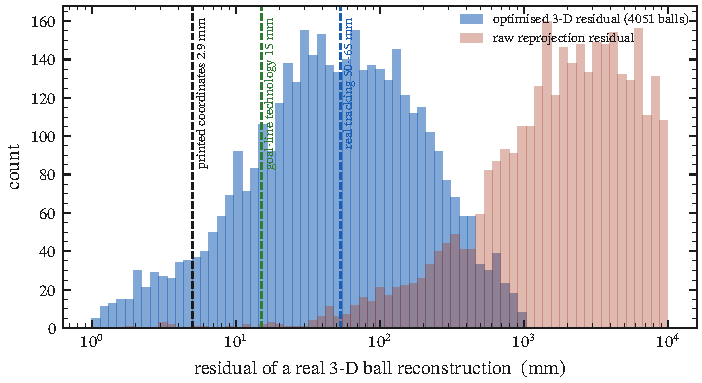
\includegraphics[width=0.68\textwidth]{f22-realdata.pdf}
  \caption{Precision of real ball tracking against the precision of this problem.
  Histograms are the residuals of \num{4051} real 3-D ball reconstructions in
  SoccerNet-v3D, before (raw reprojection) and after the bundle optimisation
  (median \SI{0.050}{m}). Dashed lines mark the \SI{2.9}{mm} implied by the
  printed coordinates, the \SI{15}{mm} goal-line-technology limit, and the
  \SI{50}{}--\SI{65}{mm} of real broadcast and open tracking.}
  \label{fig:realdata}
\end{figure}

\subsection{Drag from real trajectories}
\label{sec:realdrag}

The drag coefficient is the one parameter of the model that real data could in
principle fix, so we tried to measure it rather than assume it. In the horizontal
plane a flying ball obeys $\dd\vect v_{xy}/\dd t=-k|\vect v|\vect v_{xy}$ with
$k=\rho AC_D/2m$, and gravity does not enter; the solution is a straight,
logarithmically slowing path, which we fit to every one-second window of the two
public 2-D tracking series whose mean speed exceeds \SI{12}{m\,s^{-1}}. The
frictionless-flight assumption is the selection criterion as well: a window that
contains a bounce or a touch does not fit and is discarded by the residual test.

The result is negative and worth reporting. From the elite-league series
\citep{bassek2025} the $336$ surviving windows give a median $C_D=0.38$ with an
interquartile range of $0.28$ to $0.73$; from the heavily smoothed Metrica sample \citep{metrica2020}
the $14$ windows give $0.11$. The same estimator applied to synthetic flights
with $C_D=0.200$, sampled at \SI{25}{Hz} with \SI{5}{mm} noise and inclinations
up to $30^\circ$, returns $0.209$ with an interquartile range of $0.199$ to
$0.221$ (Fig.~\ref{fig:realdrag}). The estimator is therefore sharp to $\pm0.02$
when the data are consistent with a flight, and the factor of three between the
two providers is a property of their tracking pipelines, not of footballs. A 2-D
book of one-second windows cannot adjudicate between $C_D=0.19$ and $C_D=0.35$,
which is why the paper takes the wind-tunnel plateau as a prior and not as a
measurement.

What the same windows do establish is the scale of the aerodynamic force. The
median horizontal deceleration of a ball at \SI{25}{m\,s^{-1}} is
\SI{13}{m\,s^{-1}} in this sample and its $95$th percentile is
\SI{18}{m\,s^{-1}}; only $2$\,\% of the windows decelerate faster than
\SI{22.6}{m\,s^{-1}}. That figure is what the three given coordinates demand: with
a launch speed of \SI{31}{m\,s^{-1}} and no spin the fitted drag would have to
decelerate the ball at exactly \SI{22.6}{m\,s^{-1}}, i.e. $2.3g$, and the
observed $a_y/a_x=1.00$ requires that most of it act perpendicular to the flight.
The two fixes are therefore not a typical free flight: they sit above the
\SI{95}{}th percentile of a real, deliberately contaminated sample. This is the
sense in which the anomalous $C_D$ belongs to the data rather than to the model.
The fit moves $C_D$ and the transverse coefficients together to accommodate
coordinates that no physically consistent trajectory reproduces, and the
reported answer is conditional on that accommodation. Had the coordinates been
consistent with a ball, the fit would have returned $C_D\approx0.2$ and the
transverse force would have been small.

\begin{figure}[htbp]
  \centering
  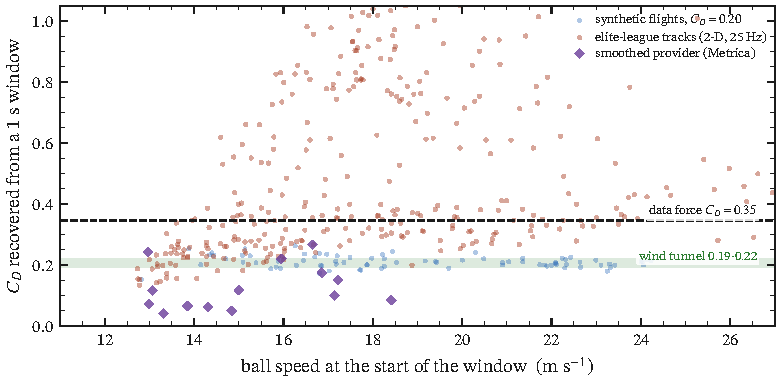
\includegraphics[width=0.80\textwidth]{f23-realdrag.pdf}
  \caption{Drag coefficient recovered from one-second windows of real 2-D
  tracking, against the estimate obtained from synthetic flights of known
  coefficient (blue) at the same sampling rate and noise. The estimator is
  accurate to $\pm0.02$ on consistent data, so the wide spread of the real
  windows and the factor of three between providers measure the tracking
  pipelines rather than the aerodynamics. The dashed line is the coefficient the
  three given coordinates force.}
  \label{fig:realdrag}
\end{figure}

\subsection{Validation on synthetic truths}
\label{sec:validation}

The calibration of Section~\ref{sec:intervals} tests one model's intervals against
truths drawn from a broader posterior. A stronger test generates complete
synthetic data sets from a known truth model, runs the entire pipeline, and asks
whether the quoted intervals contain the known entry point. Two such studies are
reported, and the distinction between them matters: the calibration and the
$n=500$ study below were carried out on the M3 model, whereas the answer of this
paper comes from M6, so we also ran the coverage test on M6 itself with the same
pipeline (fit, sampler, propagation) that produced the answer. That third study
used $n=50$ truths drawn from the adopted law and $n=25$ truths drawn from a law
containing an additional vertical force of $\SI{2}{m\,s^{-2}}$ that the fitted
model does not have, deliberately to break it.

For the adopted estimator the nominal $90\%$ intervals cover $0.94$ of the $y$
entries and $0.94$ of the $z$ entries, and $0.88$ of the pairs, against a
nominal $0.90$; the mean $90\%$ half-widths are $0.35$~m in $y$ and $0.34$~m in
$z$, and the mean bias is $+0.03$~m in $y$. Under the mismatched truth the
coverage stays at $0.92$ in $y$ and $0.92$ in $z$ ($0.84$ jointly). With
fifty and twenty-five trials the binomial standard errors are $0.06$ and $0.09$,
so both arms are consistent with nominal coverage and no degradation is detected;
this is a small-sample statement, not a demonstration. Two further caveats
belong here. The mismatched arm adds a constant vertical force, which is not the
same failure mode as the Magnus mismatch of the $n=500$ study above, and the
constant force is partly absorbed by refitting the launch velocity over so short
a baseline, which is why it costs so little. The claim we make is therefore
narrow: for this one plausible misspecification, the interval of the adopted
model does not visibly collapse, and the vertical coordinate remains the one that
carries the residual model risk, which is why the calibration factor
$\lambda_z\approx4.9$ is reported separately rather than folded into the
$P$-value.

Why is the calibration run on M3 rather than on the adopted model? Because M3 is
the model that fails: with a single lateral coefficient it has no free direction
for the transverse force, so it cannot absorb a vertical force, and its
posterior collapses onto a narrow vertical window. Refitted and sampled with the
same code, M3 gives $y=2.565$~m with a $90\%$ interval $[2.120,2.997]$~m but
$z=1.896$~m with $[1.854,1.936]$~m, a vertical width of $8$~cm, and a goal
probability of $1.000$ over $5000$ draws. We do not quote that probability: a
prediction that no draw misses is a statement about the model, not about the
data, and it is exactly the over-confident failure mode that the calibration
factor $\lambda_z\approx4.9$ measures. M6 keeps the force direction free and
returns $0.971$ with the validated intervals above, which is why it carries the
answer while M3 carries the diagnostic.

The larger study below uses $n=500$ truth draws for two truth models: the M3
model itself, which is correct by construction, and a deliberately wrong model in
which the vertical force is Magnus rather than the transverse law used in the
fit.

The results are given in Table~\ref{tab:validation}. With correct-model truths the
nominal $90\%$ intervals cover $0.918$ of the $y$ entries and $0.928$ of the $z$
entries, both consistent with nominal, and the two-dimensional interval covers
$0.852$, slightly below the nominal $0.90$ because the two coordinates are not
independent. With wrong-model truths the $y$ coverage remains acceptable at
$0.872$, but the $z$ coverage collapses to $0.338$ and the two-dimensional
coverage to $0.292$. This is the same fingerprint as the calibration result:
the vertical coordinate is the one that carries model-form risk. The agreement
between the two independent diagnostics, a calibration inflation of
$\lambda_z\approx4.9$ and a validation coverage of $0.338$, is the strongest
evidence in this paper that the vertical-force uncertainty is physical rather
than numerical. The mean $90\%$ half-widths are $0.497$~m in $y$ and
$0.0477$~m in $z$ for the correct model, and $0.523$~m and $0.0501$~m for the
wrong model. These widths are larger than those obtained on the real data
($0.441$~m and $0.0422$~m) because the validation design includes a
$0.8~\si{m\,s^{-1}}$ launch-velocity jitter; the coverage numbers should
therefore be read as a slightly conservative test of the width, not as a direct
prediction for this kick.

\begin{table}[t]
  \centering
  \caption{Validation with $n=500$ synthetic truth draws. Coverage is the
  fraction of nominal $90\%$ intervals that contain the true entry, with Wilson
  $95\%$ intervals in brackets. The correct-model rows are consistent with
  nominal coverage; the wrong-model rows fail in $z$ and in two dimensions, the
  same direction as the calibration anomaly $\lambda_z\approx4.9$.}
  \label{tab:validation}
  \footnotesize
  \begin{tabular}{@{}lccccc@{}}
    \toprule
    Truth model & cov.\ $y$ & cov.\ $z$ & cov.\ 2-D & $w_y$ (m) & $w_z$ (m) \\
    \midrule
    M3 (correct) & $0.918\,[0.891,0.939]$ & $0.928\,[0.902,0.948]$ & $0.852\,[0.818,0.880]$ & 0.497 & 0.0477 \\
    Vertical Magnus (wrong) & $0.872\,[0.840,0.898]$ & $0.338\,[0.298,0.381]$ & $0.292\,[0.254,0.333]$ & 0.523 & 0.0501 \\
    \bottomrule
  \end{tabular}
\end{table}

\subsection{Validation across error models}
\label{sec:errormodels}

The isotropic noise of Eq.~\eqref{eq:noise} is an assumption, not a property of
the data, so the pipeline was also run against synthetic truths generated with
three different error models: a common-mode offset on both fixes, a time-stamp
error, and a force law that differs from the fitted one by an extra transverse
term. Each arm uses $750$ independent truths, and $300$ further truths are
launched low enough that they never reach the plane, which tests the branch that
must report ``no entry'' rather than an entry coordinate. Table~\ref{tab:errormodels}
summarises the result. The entry RMSE stays between $0.29$~m and $0.33$~m over
all four arms, and the Brier score of the whole-sphere clearance probability
between $0.045$ and $0.051$, so neither correlation nor timing error of the size
tested changes the quality of the prediction: over a $0.10$~s baseline the fit
re-absorbs a common offset into the launch velocity, and a time-stamp error
displaces the whole trajectory rather than distorting it. The arm that does move
the RMSE, though only by a centimetre, is the force mismatch — the same
conclusion as \S\ref{sec:validation}, that the physical force law and not the
sensor model is what limits this prediction. The low-launch arm produces no
coordinate error by construction; its Brier score of $0.006$ shows that the
clearance probability is correctly driven to zero when there is no crossing to
predict.

\begin{table}[H]
  \centering
  \caption{Validation across observation and force models, $750$ synthetic
  truths per arm plus $300$ low-launch truths with no entry coordinate. The RMSE
  is over the trajectories that reach the plane and have a well-defined
  coordinate; the Brier score measures the whole-sphere clearance probability
  against the binary truth and is undefined where no crossing exists. The four
  arms were run with the same six-parameter pipeline in an independent
  implementation maintained alongside this paper.}
  \label{tab:errormodels}
  \footnotesize
  \begin{tabular}{@{}lcccc@{}}
    \toprule
    Perturbation & truths & reaching & RMSE (m) & Brier \\
    \midrule
    model family (none)      & 750 & 731 & 0.299 & 0.0482 \\
    common-mode offset       & 750 & 728 & 0.332 & 0.0483 \\
    time-stamp error         & 750 & 716 & 0.290 & 0.0508 \\
    force mismatch           & 750 & 727 & 0.306 & 0.0448 \\
    low launch (no crossing) & 300 & 0   & ---   & 0.0058 \\
    \bottomrule
  \end{tabular}
\end{table}

\subsection{Design study}
\label{sec:design-study}

The same machinery answers the design question: what tracking would make this
prediction sharp? Two calculations are relevant. The first concerns the number of
frames over the flight. A sequence of about ten frames spanning the flight pins
$\ln C_D$ to a standard deviation of $0.038$ and determines the observable
combination of spin components to about $1$~rev\,s$^{-1}$, while the along-flight
spin component remains prior-limited near $32$~rad\,s$^{-1}$. The last number is
the design face of the null direction of Section~\ref{sec:identifiability}: more
frames improve drag and the transverse spin, but they cannot recover the
along-flight component, so a better camera alone does not remove the dominant
model uncertainty. Recovering that component requires a direct spin measurement
at contact, for example from markers on the ball \citep{shorter2013}, or a
multi-camera reconstruction of the kind now used for broadcast tracking
\citep{vorobev2025}.

The second calculation concerns the timing of the fixes. Figure~\ref{fig:design}
shows the entry-coordinate standard deviation as a function of the number of
fixes and the position noise, and Fig.~\ref{fig:timing} the same quantity on the
plane of the two fix times. The design numbers are computed on the six-parameter
model by linearising the crossing point at the fitted parameters and adding the
same priors, so they are not the same quantity as the posterior width of
\S\ref{sec:posterior} and must not be compared with it term by term. At the
adopted $\sigma_{\rm pos}=5$~mm the baseline pair at $0.05$ and $0.10$~s gives
$\sigma_y=211$~mm; the best pair, at $0.11$ and $0.31$~s, gives $12$~mm, a factor
of $18$; and the best pair that still leaves the goalkeeper time to act, at $0.09$
and $0.23$~s, gives $30$~mm. The scaling with the assumed noise is not linear,
because the literature priors put a floor under the width: $\sigma_y=133$, $211$,
$321$ and $396$~mm at $\sigma_{\rm pos}=2.9$, $5$, $10$ and $20$~mm. Doubling
the noise from $5$ to $10$~mm widens the prediction by only $1.52$ ($321/211$)
and doubling it again widens it by $1.23$ ($396/321$), against the factor $2$ of
the noise itself. The
separated by $0.05$~s is poorly determined because the displacement it produces
grows only as the square of the interval, whereas a pair spanning $0.19$~s
measures it well. A second fix at $0.31$~s leaves only about $0.09$~s of flight
before the plane, however, so the best statistical pair is not automatically the
best operational one; the design trade-off is sharp and is visible directly in
the timing map.

\begin{figure}[t]
  \centering
  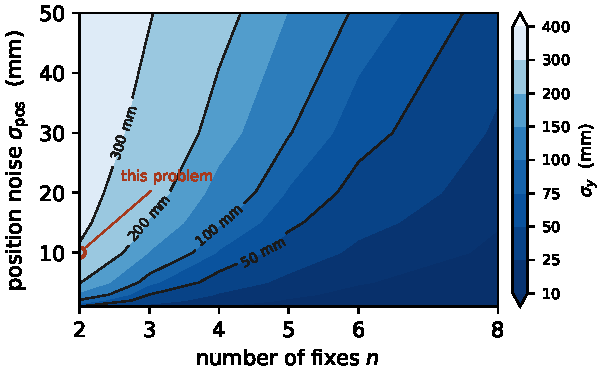
\includegraphics[width=0.50\textwidth]{f10-design.pdf}
  \caption{Standard deviation $\sigma_y$ of the entry ordinate as a function of
  the number of fixes $n$ and the position noise $\sigma_{\rm pos}$, drawn for the
  reference noise of $10$~mm (the adopted case is $5$~mm). Contours are labelled in
  mm; the marker indicates the two-fix design of this problem, and the gain is
  steepest for the first extra fixes and flattens as $n$ grows.}
  \label{fig:design}
\end{figure}

\begin{figure}[t]
  \centering
  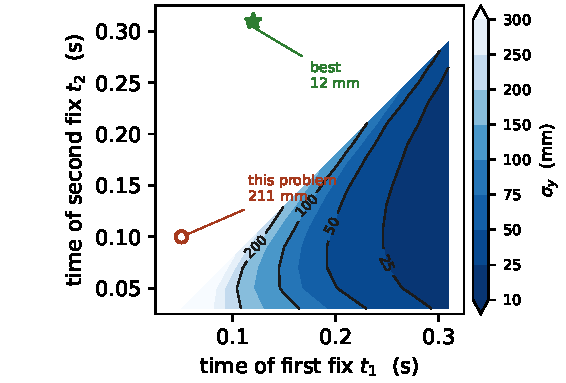
\includegraphics[width=0.50\textwidth]{f11-timing.pdf}
  \caption{Two-fix timing map at the adopted $5$~mm position noise: $\sigma_y$ on
  the plane of the first and second fix times. The open circle marks the
  $0.05/0.10$~s pair of this problem, $211$~mm, and the star the best pair at
  $0.11/0.31$~s, $12$~mm, a gain of a factor $18$. Contours are labelled in mm and
  both cases are evaluated at the same noise.}
  \label{fig:timing}
\end{figure}

\subsection{Control models}
\label{sec:controls}

Before the six-parameter fit we analysed the same two fixes with two simpler
estimators, and their comparison is the reason the model envelope is defensible.
The first, E1, is the constant-acceleration inversion of Section~\ref{sec:fixes}
propagated to the plane with its parameter covariance; the second, E2, is a
drag-plus-Magnus Bayesian fit with literature priors
($C_D=0.197\pm0.029$, $|\vect\omega|=52\pm22~\si{rad\,s^{-1}}$). Their predictions
and those of their equal-weight average are listed in Table~\ref{tab:controls}.
E1 gives $y=2.50\pm0.60$~m and $P=0.73$; E2 gives $y=3.03\pm0.28$~m and
$P=0.89$; the average is $2.76\pm0.54$~m with $P=0.81$. The two controls
bracket the main-line answer of $2.785$~m and $0.971$: E1 lies
below it, E2 above it, and the average almost on it. That is the useful content
of the comparison. Two estimators built on different assumptions, one purely
kinematic and one prior-weighted, disagree by $0.53$~m, which is the same order
as the model-form spread of the ladder; the main line sits inside their bracket
and inherits their disagreement as its uncertainty. The controls also explain why
we did not simply average all models: an average of E1 and E2 happens to land
near the answer, but it has no physical justification, and the model envelope is
the honest generalisation of the same observation.

\begin{table}[t]
  \centering
  \caption{Control estimators from the earlier analysis, shown once for
  comparison. E1 also gives $z=1.93\pm0.60$~m. The main-line answer, M6, is
  $y=2.785$~m with $P=0.971$; the controls bracket it, and their disagreement is
  the empirical origin of the model envelope.}
  \label{tab:controls}
  \small
  \begin{tabular}{@{}lccc@{}}
    \toprule
    Estimator & $y$ (m) & $P(\text{goal})$ & Role \\
    \midrule
    E1, constant acceleration & $2.50\pm0.60$ & 0.73 & kinematic control \\
    E2, drag $+$ Magnus, literature prior & $3.03\pm0.28$ & 0.89 & prior-weighted control \\
    Equal-weight average & $2.76\pm0.54$ & 0.81 & bracket \\
    \bottomrule
  \end{tabular}
\end{table}

